\documentclass[a4paper,10pt]{article}
\usepackage[USenglish,ngerman,english]{babel} %francais, polish, spanish, ...
\usepackage[T1]{fontenc}
\usepackage[ansinew]{inputenc}
\usepackage{lmodern} %Type1-font for non-english texts and characters
\usepackage[parfill]{parskip}

%% Watermark     %%%%%%%%%%%%%%%%%%%%%%%%%%%%%%%%%%%%%%%%%%%%%
%\usepackage{draftwatermark}		 % watermark on every page
\usepackage[firstpage]{draftwatermark}  % watermark only on first page
%\usepackage[nostamp]{draftwatermark}	 % quickly removes watermark

%% Math          %%%%%%%%%%%%%%%%%%%%%%%%%%%%%%%%%%%%%%%%%%%%%
\usepackage{amsmath,amssymb}

%% Tables 	 %%%%%%%%%%%%%%%%%%%%%%%%%%%%%%%%%%%%%%%%%%%%%
\usepackage{array}
\newcolumntype{L}[1]{>{\raggedright\let\newline\\\arraybackslash\hspace{0pt}}m{#1}} % column with 
\usepackage{booktabs}
\usepackage{tabularx}
\usepackage{longtable}
%\usepackage{ctable}

%% Layout 	 %%%%%%%%%%%%%%%%%%%%%%%%%%%%%%%%%%%%%%%%%%%%%
%\usepackage[left=2.5cm,right=2.5cm,top=2.5cm,bottom=2.5cm,includeheadfoot]{geometry}
\usepackage{geometry}
\usepackage{xcolor,colortbl}
\usepackage{graphicx}
\usepackage[font=normalsize]{caption}
\usepackage{color} % needed for background color in listings
\definecolor{Gray}{gray}{0.85}
\usepackage[ 
    colorlinks,        % Links ohne Umrandungen in zu wählender Farbe 
    linkcolor=black,   % Farbe interner Verweise 
    filecolor=black,   % Farbe externer Verweise 
    citecolor=black,   % Farbe von Zitaten 
    urlcolor =black    % Farbe von Links
]{hyperref}
\usepackage{float}
\usepackage{cite}
\usepackage{apacite}

% cpations for figures and tables
\captionsetup[table]{
	format=plain,
	labelformat=simple,
	labelsep=newline,
	justification=raggedright,
	singlelinecheck=false,
	labelfont={bf},
	textfont={sl,small},
	aboveskip= 5pt,
	belowskip= 5pt} 
\captionsetup[figure]{
	format=hang,
	labelformat=simple,
	labelsep=colon,
	justification=justified,
	singlelinecheck=false,
	labelfont={bf},
	textfont={rm,small},
	parskip=5pt,
	aboveskip= 10pt,
	belowskip= 10pt}
	
% appearance of the watermark
%\SetWatermarkAngle{} % Angle at which the watermark text is drawn
%\SetWatermarkColor[rgb]{0,1,0} % can also be used as {colorname}
\SetWatermarkLightness{0.9} % Lightness of the watermark text (1=white, 0=black), this just sets a value for the grey
\SetWatermarkFontSize{4cm} % Font size of the watermark text
%\SetWatermarkScale{} % Scaling of the watermark text
\SetWatermarkText{beta version} % Watermark text
	

%% Line Spacing %%%%%%%%%%%%%%%%%%%%%%%%%%%%%%%%%%%%%%%%%%%%%
\usepackage{setspace}
\singlespacing        %% 1-spacing (default)
%\onehalfspacing       %% 1,5-spacing
%\doublespacing        %% 2-spacing

%% Listings     %%%%%%%%%%%%%%%%%%%%%%%%%%%%%%%%%%%%%%%%%%%%%
\usepackage{listings}
\usepackage{listing}
% layout for MATLAB listings used in the TRENTOOL documentation

% define colors used in listings
\definecolor{lightgray}{RGB}{230,230,230}
\definecolor{lightyellow}{RGB}{252,245,224}
\definecolor{keyblue}{RGB}{20,7,252}
\definecolor{commentgreen}{RGB}{83,133,50}
\definecolor{stringpink}{RGB}{197,73,205}

% FONTS:
%\textrm{..}	 \rmfamily	 R�misch
%\textit{..}	 \itshape	 Schr�ger Text (auch \emph{})
%\textbf{..}	 \bfseries	 Fetter Text
%\textsc{..}	 \scshape	 Text in Kapit�lchen
%\texttt{..}	 \ttfamily	 Schreibmaschinentext
%\textnormal{..}	 \normalfont	 Standardfont im Dokument

\lstset{
basicstyle=\footnotesize\ttfamily, 
keywordstyle=\bfseries\color{keyblue},
commentstyle=\color{commentgreen},
stringstyle=\color{stringpink},
numbers=left,                   % where to put the line-numbers
numberstyle=\tiny,      % the size of the fonts that are used for the line-numbers
stepnumber=1,                   % the step between two line-numbers. If it's 1, each line 
numbersep=5pt,                  % how far the line-numbers are from the code
backgroundcolor=\color{lightyellow},  % choose the background color. You must add \usepackage{color}
showspaces=false,
breaklines=true,
}

%\lstset{ %
%language=Matlab,                % the language of the code
%basicstyle=\footnotesize       % the size of the fonts that are used for the code
%basicstyle=\scriptsize\ttfamily,

%keywordstyle=\bfseries,\color{blue},
%identifierstyle=,
%commentstyle=\color{lightgray},	
%stringstyle=\itshape\color{magenta},
%
%numbers=left,                   % where to put the line-numbers
%numberstyle=\tiny,      % the size of the fonts that are used for the line-numbers
%stepnumber=1,                   % the step between two line-numbers. If it's 1, each line 
%                                % will be numbered
%numbersep=5pt,                  % how far the line-numbers are from the code
%backgroundcolor=\color{lightgray},  % choose the background color. You must add \usepackage{color}
%showspaces=false,               % show spaces adding particular underscores
%showstringspaces=false,         % underline spaces within strings
%showtabs=false,                 % show tabs within strings adding particular underscores
%%frame=single,                   % adds a frame around the code
%tabsize=2,                      % sets default tabsize to 2 spaces
%captionpos=t,                   % sets the caption-position to bottom
%breaklines=true,                % sets automatic line breaking
%breakatwhitespace=false,        % sets if automatic breaks should only happen at whitespace
%%title=\lstname,                 % show the filename of files included with \lstinputlisting;
%                                % also try caption instead of title
%escapeinside={\%*}{*)},         % if you want to add a comment within your code
%morekeywords={*,...},            % if you want to add more keywords to the set
%float=H,
%}

\newcommand{\origttfamily}{}
\let\origttfamily=\ttfamily %Voheriges \ttfamily sichern
\renewcommand{\ttfamily}{\origttfamily \hyphenchar\font=`\_}


\begin{document}
%opening
\title{TRENTOOL 3.1 -- Using the Ragwitz Criterion in TRENTOOL}
%\author{Patricia Wollstadt}
\author{Patricia Wollstadt\thanks{\texttt{p.wollstadt@stud.uni-frankfurt.de}} \and Michael Lindner \and Raul Vicente \and Michael Wibral \and Nicu Pampu \and Mario Martinez-Zarzuela}
\date{Version 1.00\\ 
\texttt{http://www.trentool.de/}}

\maketitle

%\newpage

\paragraph*{What is TRENTOOL?} TRENTOOL (\underline{TR}ansfer \underline{EN}tropy \underline{TOOL}box) is an open-source MATLAB toolbox that allows the user to easily handle the considerable complexity of transfer entropy (TE) estimation from time series. For the use with neural data TRENTOOL seamlessly integrates with the popular FieldTrip toolbox \cite{oostenveld2011}. 

\paragraph*{State Space Reconstruction} TE estimation requires the reconstruction of the state space from a scalar time series. A state is defined as the collection of random variables that uniquely describe the state of a process. The set of all possible realizations of such state variables is called the state space of the process. State spaces can be (appropriatively) reconstructed using a time-delayed embedding \cite{takens1981}, such that reconstructed states take the form 

\[
    \mathbf{x}_t^{d_x} = \left(x_t, x_{t-1}, \ldots, x_{t-(d-1)\tau} \right),
\]

where $d$ is called the embedding dimension and $\tau$ the embedding delay. To find optimal values for $d$ and $\tau$, TRENTOOL tests how well user provided pairs of candidate values for $d$ and $\tau$ optimize a local predictor \cite{ragwitz2002}. This is done in the function \texttt{TEprepare.m}

\paragraph*{The Ragwitz Criterion} We call the dimension $d$ and embedding delay $\tau$ the embedding parameters. Embedding parameters are found by optimizing a local predictor proposed in \cite{ragwitz2002}. The Ragwitz criterion uses candidate values for $d$ and $\tau$ and tests how well these candidate values embed the time series (Fig. \ref{fig:embedding}), such that for each time point the next point in time can be predicted with minimum error (Fig. \ref{fig:ragwitz}).


\begin{figure}[H]	
	\centering 
 		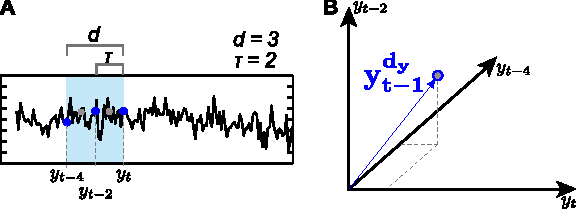
\includegraphics{ragwitz_01.pdf}
	\caption[Time-delayed embedding]{\textbf{Time-delayed embedding.} Example for the dime-delayed embedding of a point at time $t$ using embedding parameters $d=3$ and $\tau=2$. Scalar time points at times $t$, $t-2$, and $t-4$ (A) are combined into an time-delayed embedded vector (B).}
	\label{fig:embedding}
\end{figure} 

The Ragwitz criterion proceedes as follows (Fig. \ref{fig:ragwitz}):

For all pairs of candidate values $d$ and $\tau$ do the following:
\begin{enumerate}
 \item Embed the time series using $d$ and $\tau$
 \item Do the following for each embedded point $\mathbf{y_t^{d_y}}$:
 \begin{enumerate}
  \item conduct a nearest neighbour search
  \item predict the next point $\mathbf{\hat{y}_{t+1}^{d_y}}$ as the average of the nearest neighbours
  \item calculate the local error $e_t = \mathbf{\hat{y}_{t+1}^{d_y}} - \mathbf{y_{t+1}^{d_y}}$
 \end{enumerate}
 \item Sum the local errors over all embedded points
\end{enumerate}

As output, the Ragwitz criterion will return the pair of values $d$ and $\tau$, that minimize the error over all embedded time points. 


\begin{figure}[H]	
	\centering 
 		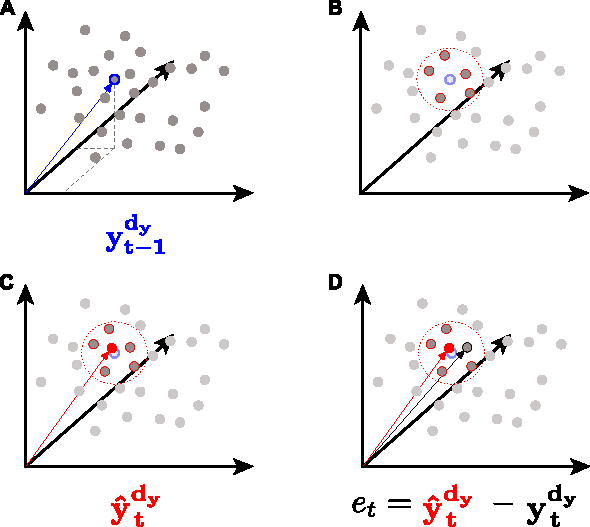
\includegraphics{ragwitz_02.pdf}
	\caption[Ragwitz Criterion]{\textbf{Ragwitz Criterion.} (A) Each point in the time series is embedded using the current values for $d$ and $\tau$. (B) A nearest neighbour search is performed for each point. (C) For each point, the next point in time is predicted as the average of the reference point's nearest neighbours. The prediction error is computed as the distance of the predicted and the actual next point.}
	\label{fig:ragwitz}
\end{figure} 


\paragraph*{Using the Ragwitz Criterion in TRENTOOL} See table \ref{tab:tab_cfgTEP} for parameters that define the behaviour of the Ragwitz Criterion in TRENTOOL. TRENTOOL requires the user to provide candidate values for $d$ and $\tau$ to use the Ragwitz Criterion for parameter optimization (parameters  \texttt{cfgTEP.ragdim} and \texttt{cfgTEP.ragtaurange} respectively). Note, that $\tau$ is given as a factor to be multiplied with the autocorrelation time (ACT) of the time series. For example, \texttt{cfgTEP.ragtaurange = [0.2 0.5]} would scan $\tau$ values from 20~\% to 50~\% of the ACT of the time series. The number of steps within the \texttt{ragtaurange} is specified in \texttt{ragtausteps}. 

TRENTOOL further allows to specify the type of neighbour search to be conducted for local prediction. The user may chose from a range search \texttt{cfgTEP.flagNei = 'Range'} or a k-Nearest-Neighbour search \texttt{cfgTEP.flagNei = 'Mass'}. Accordingly, the parameter  \texttt{cfgTEP.sizeNei} has to either define the range to be searched or the number of nearest neighbours. 

As a last parameter, the user can set the number of points to be used for local prediction in \texttt{cfgTEP.repPred}. TRENTOOL will use the first \texttt{repPred} values to predict the next point in time from nearest neighbours and to calculate the prediction error.


\begin{table}[H]
\small
\caption[Parameters \texttt{cfgTEP}]{Prameters for the configuration structure \texttt{cfgTEP.} specific to the use of the Ragwitz Criterion for embedding parameter optimization (TRENTOOL Version 3.0).} 
\makebox[\textwidth]{
\begin{tabularx}{1.1\textwidth}{lL{1.3cm}p{1.1cm}X}\toprule 
\label{tab:cfgTEP}
\textbf{field name} & \textbf{data type} & \textbf{units} & \textbf{description} \\ \midrule

\rowcolor{Gray}
\verb+optimizemethod+ & string & & define method for parameter optimization: 'ragwitz' \\%or 'cao'\\
\verb+ragdim+ & integer & samples & candidate embedding dimensions to be scanned\\
\rowcolor{Gray}
\verb+ragtaurange+ & double & units of act & 1x2-vector of min and max embedding delays \\
\verb+ragtausteps+ & integer & & number of equidistant steps in ragtaurange with a minimum of 5\\
\rowcolor{Gray}
\verb+flagNei+ & string & &'Range' or 'Mass' (kNN) type of neighbor search\\
\verb+sizeNei+ & integer & & Radius or mass for the neighbor search depending on \verb+flagNei+\\
\rowcolor{Gray}
\verb+repPred+ & integer & samples & number of sample points for which the prediction is performed (has to be smaller than $length(timeSeries)-(embedding dimension-1)*tau*ACT-u$ )\\ \bottomrule
% \multicolumn{5}{l}{}\\
% \multicolumn{5}{l}{\textbf{Parameters needed for the use of Cao criterion for parameter optimization$^{a}$}}\\ \midrule
% \verb+caodim+ & \verb+1 to 10+ & integer & & for Cao: indicates the range of dimensions that is scanned using the Cao criterion to find the optimal dimension \\
% \rowcolor{Gray}
% \verb+caokth_neighbors+ & \verb+4+ & integer & & for Cao: number of neighbors for fixed mass search for cao (controls balance of bias/statistical errors) \\
% \verb+tau+ & \verb+1.5+ & double & units of act & for Cao: embedding delay \\ 
% \multicolumn{5}{p{\textwidth}}{$^a$ The cao criterion is not recommended for parameter optimization. The code for cao-optimization is no longer maintained and guaranteed to work vor TRENTOOL versions 3.0 and higher.}
\end{tabularx}}
\end{table}


\bibliographystyle{apacite}
\bibliography{../DocumentationBib}

\end{document}
